%% ------------------------------------------------------------------------- %%n
\chapter{Plano de Trabalho e Cronograma}
\label{cap:Cronogramanotes}

Os créditos em disciplinas necessários para o programa de mestrado em Ciência da Computação
no IME-USP foram cumpridos de fevereiro de 2016 até junho de 2018, conforme a tabela: 

\begin{center}
\begin{tabular}{ |l|l|l| } 
\hline
\textbf{Código} & \textbf{Disciplina}                                   & \textbf{Término} \\ 
\hline
MAC5710     & Estrutura de Dados e sua Manipulação (Aluno Especial)     & 10/06/2016       \\
MAC4722     & Linguagens, Autômatos e Computabilidade                   & 30/06/2017       \\
MAC6910     & Metodologia de Pesquisa para Ciência da Computação        & 30/06/2017       \\
MAC5749     & Análise e Reconhecimento de Formas: Teoria e Prática      & 24/11/2017       \\
MAC5861     & Modelagem de Banco de Dados                               & 24/11/2017       \\
MAC5832     & Aprendizagem de Máquina: Modelos, Algoritmos e Aplicações & 22/06/2018       \\
\hline
\end{tabular}
% \label{tab:disciplinas}
\end{center}

\section{Plano de Trabalho}
\label{sec:Plano_de_Trabalho}

O plano de trabalho será composto nas seguintes tarefas:

\begin{enumerate}
  \item Estudo de trabalhos existentes com framework entre participação ativa do usuário e Aprendizado Ativo;
  \item Estudo e Implementação de diferentes frameworks de Aprendizado Ativo;
  \item Ciar ferramenta de Aprendizado Ativo com participação ativa do usuário;
  \item Fazer testes no laboratório com especialistas do Instituto de Oceanográfico da USP (IO-USO);
  \item Escrever dissertação e Defesa do Mestrado.
\end{enumerate}


\section{Cronograma}
\label{sec:cronograma}


\begin{figure}
  \centering
  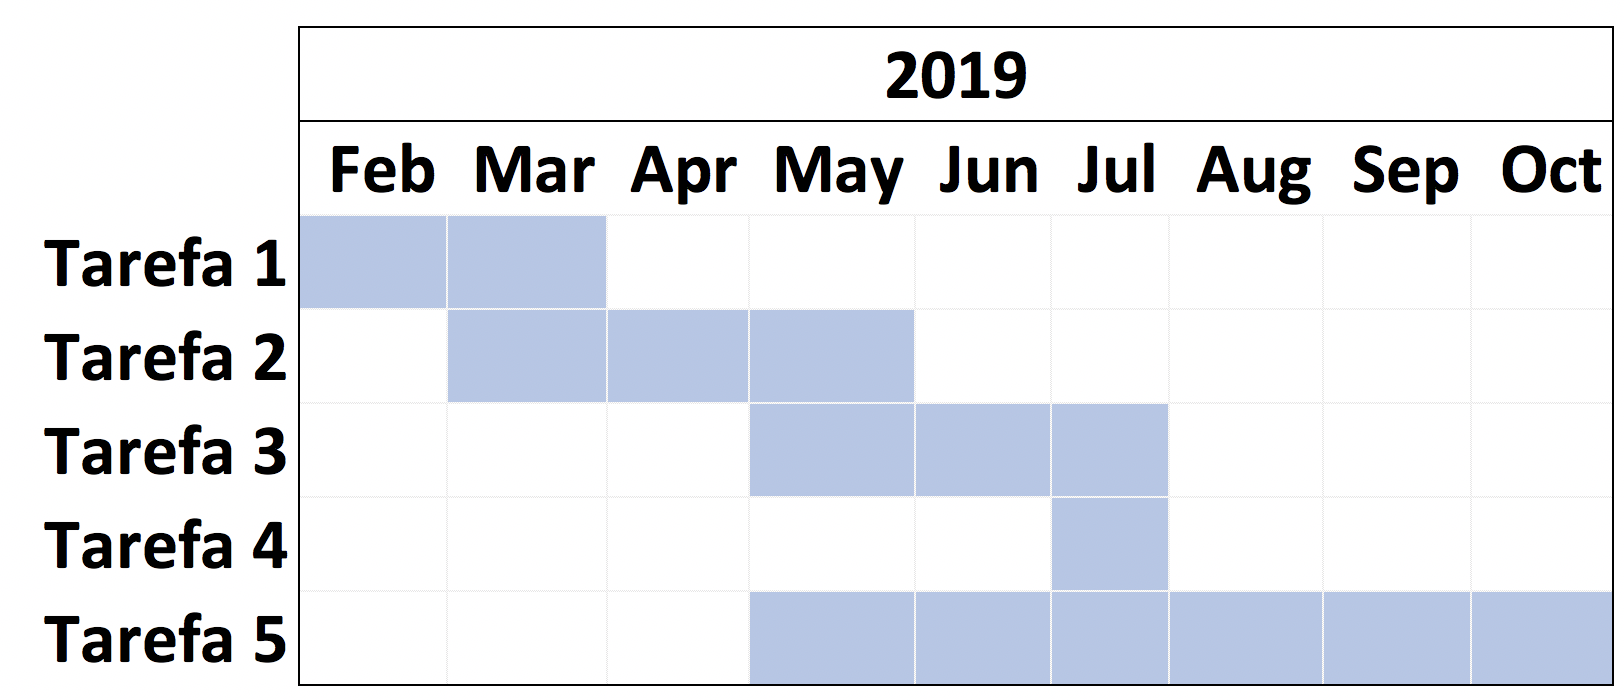
\includegraphics[width=0.4\textwidth]{figures/cronograma.png}
  \caption{Cronograma Mestrado.}
  \label{fig:cronograma}
\end{figure}
